\documentclass[12pt]{article}
\usepackage{times,mathptm}
\usepackage{graphicx}
\usepackage{anysize}
\usepackage{amsmath}
\usepackage{color}
\usepackage{fancyhdr}

%% Set Variables % (fold)
\newcommand{\setto}[1]{\def\varto{#1}}
\newcommand{\setfrom}[1]{\def\varfrom{#1}}
\newcommand{\setdate}[1]{\def\vardate{#1}}
\newcommand{\setsubject}[1]{\def\varsubject{#1}}
\newcommand{\setcc}[1]{\def\varcc{#1}}
%% End Set Variables (end)
%% Make Obejcts (fold)
\newcommand{\makeheader}{
\begin{tabular}{ll}
\textbf{To:} & \varto \\ \\
\textbf{From:} & \varfrom \\ \\
\textbf{Date:} & \vardate \\ \\
\textbf{Subject:} & \varsubject \\ \\
\textbf{CC:} & \varcc \\ \\
\end{tabular}}
%% End Make Objects (end)
%% Make New Lines (fold)
\newcommand{\newversionline}[4]{\parbox{.42in}{#1}&\parbox{1.25in}{#2}&\parbox{1in}{#3}&\parbox{2.5in}{#4}\\ \vspace{3pt}}
\newcommand{\newrequirementclass}[3]{\newcounter{#2}\setcounter{#2}{1}\parbox{1.5in}{#1}&\parbox{.75in}{#2}&\parbox{3.5in}{#3}\\ \vspace{3pt}}
\newcommand{\newrequirementbox}[4]{\framebox{\parbox{6.17in}{
\hspace{3pt}\parbox{6.17in}{\parbox{2in}{\textbf{Number:} #1-\arabic{#1}}
\textbf{Name:} \parbox{3.17in}{#2}\vspace{6pt}}\\\vspace{6pt}
\parbox{6.17in}{\textbf{Description:} #3}\\\vspace{6pt}
\parbox{6.17in}{\textbf{Verification Method:} #4}}}
\stepcounter{#1}\vspace{12pt}}
\newcommand{\newrequirementnotes}[5]{\framebox{\parbox{6.17in}{
\hspace{3pt}\parbox{6.17in}{\parbox{2in}{\textbf{Number:} #1-\arabic{#1}}
\textbf{Name:} \parbox{3.17in}{#2}\vspace{6pt}}\\\vspace{6pt}
\parbox{6.17in}{\textbf{Description:} #3}\\\vspace{6pt}
\parbox{6.17in}{\textbf{Verification Method:} #4}\\\vspace{6pt}
\parbox{6.17in}{\textbf{Notes:} #5}}}
\stepcounter{#1}\vspace{12pt}}
\newcommand{\newriskbox}[4]{\framebox{\parbox{6.17in}{
\textbf{Description:} \parbox{5in}{#1}\vspace{3pt}

\textbf{Detection:} \parbox{5in}{#2}\vspace{3pt}

\textbf{Mitigation Plan:} \parbox{5in}{#3}\vspace{3pt}

\textbf{Avoidance:} \parbox{5in}{#4}}}\vspace{12pt}}
%% End Make New Lines (end)
%% Custom Environments (fold)
\newenvironment{overview}{\vspace{12pt}\begin{center}\begin{minipage}[c]{5in}\footnotesize\begin{center}\textbf{Overview}\end{center}}{\end{minipage}\end{center}\vspace{12pt}}
\newenvironment{versionbox}{\begin{center}\textbf{Version}\end{center}\footnotesize\begin{tabular}{llll}
Version & Date and Time & Sign Off & Changes Made \\ \hline}{\end{tabular}}
\newenvironment{requirements}{\begin{tabular}{lll}
\parbox{1.5in}{Type of Requirement}&\parbox{.75in}{Label}&\parbox{3.5in}{Description}\\ \hline \vspace{3pt}}{\end{tabular} \\}
%% End Custom Environments (end)
\setlength{\parindent}{0pt}
\setdate{\today}

%% Fancy Header (fold)
\marginsize{1in}{1in}{1in}{1in}
\pagestyle{fancy}
\fancyhead{}
\fancyfoot{}
\fancyhead[RO,RE]{Software Requirements Specification}
\fancyhead[LO,LE]{Split-Dev}
\fancyfoot[CO,CE]{\thepage}
%% End Fancy Header (end)
\renewcommand{\headrulewidth}{0.8pt}
\renewcommand{\footrulewidth}{0pt}

%% Title
\title{\textbf{Split}}
\author{2260 Hayward \\
Ann Arbor, MI 48109}
\date{\today}
%% Header
\setto{Rod Johnson, Instructor, University of Michigan}
\setfrom{Split-Dev \\
 & Jim Brusstar, Developer \\
 & Michael Lee, Developer \\
 & Ben Montgomery, Developer \\
 & Robert Steen, Developer
}
\setsubject{Software Requirements Specification}
\setcc{Elliot Solloway, Instructor, University of Michigan}

\begin{document}

\maketitle

\makeheader

\begin{versionbox}
\newversionline{0.1}{5 Oct 2009 4:30pm}{mzlee, rdsteen}{Initial draft - overview, project management}
\newversionline{0.2}{8 Oct 2009 4:30 pm}{mzlee, rdsteen}{Condensed project definition, requirements}
\newversionline{0.3}{9 Oct 2009 3:30 pm}{benmonty, mzlee, jimbru}{Added non functional requirements}
\newversionline{0.4}{11 Oct 2009 7:00 pm}{mzlee}{Fixed formatting and added project management}
\newversionline{0.5}{11 Oct 2009 9:00 pm}{benmonty}{Corrected wording, removed underlines, added comments}
\newversionline{1.0}{12 Oct 2009 12:40 pm}{mzlee}{Merged conflicting project definition paragraph}
\newversionline{1.1}{21 Oct 2009 6:30 pm}{mzlee}{Start port to \LaTeX}
\newversionline{1.2}{23 Oct 2009 3:00 am}{mzlee}{Finished port to \LaTeX}
\newversionline{1.3}{23 Oct 2009 3:00 pm}{mzlee, rdsteen}{Added functional requirements}
\end{versionbox}
\section*{Overview} % (fold)
\label{sec:overview}
Today, most people use tabbed web browsers to access information online. Using tabs increases efficiency and allows a user to view web content more effectively; however, the power of tabbed browsing has reached a limit. The amount of information amassed in a browsing session has become too much for a user to easily control. We are proposing a new style of browsing that allows users to crop their browser windows into exactly what they want to see. This document defines in more detail what our project is and how we will accomplish it. The project definition provides background about the project, objectives, and stakeholders; the technical issues cover an analysis of our user base, stricter definitions of our requirements, and a list of open issues in the form of risks and mitigations.
% section Overview (end)
\section{Project Definition} % (fold)
\label{sec:project_definition}
Web browsers have been an ever-evolving form of communication and information distribution. They have evolved from the old days of AOL, with the single box and cascading screens to Internet Explorer, which allowed for many windows in a desktop and now to Firefox, with tabbed browsing. We are now reaching the point of information saturation where none of these models is efficient enough. The biggest problem is that it is not the user who really decides what he or she wants to see; it's the content provider. You may be able choose to look at whatever pages you want, but do you do not have control over the ads, flash, and other distractions. We will create a platform that allows users to decide what they want to see and how they want to see it. \\

The objective of this project is to create a proof of concept system to demonstrate our technology and its usefulness in the web browser space. It is not to try to actively compete with other web browsers, that market is already saturated. Instead, we wish to show innovation so that we may be able to patent and later develop a better business model. The primary stakeholders of this project are our team members as we will be investing the time, energy, and work into the project. Additionally, the end users will have some stake in our continued development and innovation after our first alpha release. Finally, the University will have a marginal stake in our success as our success leads to furthering the reputation of the University of Michigan.
% section Project Definition (end)
\section{Technical Issues} % (fold)
\label{sec:technical_issues}
\subsection{User Analysis} % (fold)
\label{sub:user_analysis}
\emph{Power Users}

Power users are our primary demographic. These are the people who want to get as much out of their time as possible when it comes to using a web browser. They will be the people who often want to reorganize their data; the ones who will want a history of clips and positions. They will be our strongest demographic and will be the set of people who will evangelize our product. \\

\emph{Casual Users}

Casual users want to just have a web browser and may occasionally use the added functionality of being able to split a page. Usually this person will be introduced to the product by a friend (and power user) who will likely set up defaults. The casual user's experience will entail the use of the defaults to check back to a set of initial pages.

% subsection user_analysis (end)
\subsection{Requirements Definition} % (fold)
\label{sub:requirements_definition}
This requirements enumeration has been divided into different groups. The numbering scheme uses the following group labels, and all requirements will fit into one of these categories. \\

\begin{requirements}
\newrequirementclass{User}{USR}{Requirements affecting how the program appears to the user}
\newrequirementclass{Implementation}{IMP}{Requirements that provide the program’s standard functionality}
\newrequirementclass{Performance}{PERF}{Requirements that affect the program’s performance}
\end{requirements}

\newrequirementbox{IMP}{Render Mask}
{Technical Requirement. The browser must be able to define a render mask for clipping purposes.}
{Test cases will be used to ensure that a render mask can be defined.}

\newrequirementbox{IMP}{Incorporate WebKit}
{Technical Requirement. Incorporate open source technologies to help our development process and not re-implement a widely available technology.}
{Code base must rely on WebKit.}

\newrequirementbox{IMP}{Adhere to HTML Standards}
{Technical Requirement. We must adhere to web standards in our render and display. We want to not fragment the web by introducing new HTML tags.}
{Self enforced. We depend on WebKit to adhere to web standards and will self enforce ourselves to not add new structures.}

\newrequirementbox{IMP}{Open a Browser Window}
{Functional Requirement. Users will be able to open a new default browser window.}
{Test a mechanism that opens a new browser window.}

\newrequirementbox{IMP}{Navigate to a Web Page}
{Functional Requirement. Users will be able to navigate from one page to another.}
{Navigate the web browser through a sequence of pages.}

\newrequirementbox{IMP}{Basic Web Navigation}
{Functional Requirement. User should be able to open a new window and navigate to a web page.}
{Navigate between various webpages and follow a string of test links.}

\newrequirementbox{IMP}{Enter Clipping Mode}
{Functional Requirement. When viewing a default browser window, users will be able to enter clipping mode. Here they will be able to select areas of content which they wish to view.}
{Have a mechanism that allows entry into clipping mode. Test to make sure selection works.}

\newrequirementbox{IMP}{Exit Clipping Mode}
{Functional Requirement. After making selections in clipping mode, user will be able to hide the rest of the content.}
{Test to make sure when exiting clipping mode that the visible area is the area selected and the rest is masked.}

\newrequirementbox{IMP}{Clip Object Control}
{Functional Requirement. When a clip is selected, users should be able to maximize to the full page, minimize, close, and move the crop.}
{Test user inputs to verify functionality exists.  Create a set of test cases to check for corner cases.}

\newrequirementbox{IMP}{Advanced Web Navigation}
{Functional Requirement. When viewing a full page, users will be able to navigate backwards and forwards within the sequence of sites they have visited.}
{Navigate through different webpages and verify that history is preserved.}

\newrequirementbox{USR}{Usable Interface}
{Non-functional Requirement. The interface provided for the web browser must be considered simple to use.}
{A Usability study will be performed, where an average score of 7 out of 10 is required for this requirement to be met.}

\newrequirementbox{USR}{Render Mask Interface}
{Non-functional Requirement. The browser must have a user-accessible interface for defining a render mask.}
{A Usability study will be performed, where an average score of 7 out of 10 is required for this requirement to be met.}

\newrequirementbox{PERF}{Availability}
{Non-functional Requirement. The software must be available to users for download.}
{The software will be able to be downloaded from some server connected to the internet.}

\newrequirementbox{PERF}{Demonstrability}
{Non-functional Requirement. It must be possible to successfully demonstrate the capabilities of the browser to interested users.}
{The development team will demonstrate the project twice over the course of the semester.}

\newrequirementbox{PERF}{Distributable}
{Non-functional Requirement. The software must be packaged in a way such that it is easy to transport from computer to computer.}
{The browser and all other components will be combined and possibly compressed into a single file for distribution.}

\newrequirementnotes{PERF}{Portability}
{Non-functional Requirement. The browser must be able to run on Microsoft, Apple, and Linux operating systems.}
{The development team will run the browser on each of the operating systems.}
{Both WebKit and QT are cross platform and therefore portable.}

\newrequirementbox{PERF}{Responsiveness}
{Non-functional Requirement. The Split modifications should not slow the browsing experience noticeably in any way.}
{Test different browsers on the same computer and use a human to detect any reductions in speed.}

\newrequirementbox{PERF}{Safety}
{Non-functional Requirement. Split modifications must not break the browser security model.}
{Perform a basic security review and ask an external partner for a security review of our product.}

\newrequirementbox{PERF}{Simplicity}
{Non-functional Requirement. The average user must be able to quickly pick up and start using the clipping technology.}
{Perform a usability study where a user begins with no knowledge of the software and is required to perform a set of clipping tasks.}

\newrequirementnotes{PERF}{Testability}
{Non-functional Requirement. Developers must be able to easily write and run tests on the software.}
{Create use case tests and automated functionality tests}
{Both WebKit and QT have built in test cases we can reuse.}
% subsection requirements_definition (end)
\subsection{Risks} % (fold)
\label{sub:risks}
Below we have listed our major risks to the project, our detection method, possible mitigations, and our avoidance plans. Because the technology we are trying to implement is largely unexplored, we do not have very many known risks; however the ones we are aware of are potentially project defining. \\

\newriskbox{May not have enough time to complete fully functional browser}
{Periodically compare current status to roadmap}
{Use a publicly available, pre-made web browser}
{Weekly status meetings}

\newriskbox{Could compromise browser security model}
{Ask for an external security review}
{Create a new security model for our browser}
{Do not alter core browser functionality}

\newriskbox{Technology used is not capable of performing required tasks}
{Exploring the functionality and documentation of Qt and WebKit}
{UI frameworks and web rendering engines are interchangeable}
{Sought professional advice before beginning}
% subsection risks (end)
% section technical_issues (end)
\section{Project Management} % (fold)
\label{sec:project_management}
\subsection{Schedule} % (fold)
\label{sub:schedule}
Our tentative plan is displayed in figure \ref{fig:roadmap}. As you can see, we have decided to break down the work items into approximately four-week sprints. We have begun work on our system and are currently on target with our projections. \\

After our initial research task, we have discovered that there is very little to do in WebKit and most of our time will be spent in UI development using QT. The project breakdown remains the same.
% subsection schedule (end)
\begin{figure}[htp]
\centering
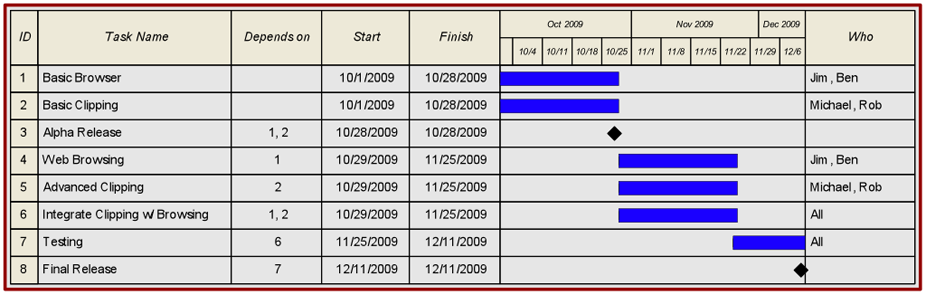
\includegraphics{RoadMap.png}
\caption[Tentative Schedule]{The Tentative Schedule}\label{fig:roadmap}
\end{figure}
\subsection{Resources} % (fold)
\label{sub:resources}
Every member of our team is a skilled programmer and will, in that capacity, be an invaluable asset. Some members of our team have more specialized backgrounds that will be of assistance. Jim Brusstar and Ben Montgomery have done prior work on user interfaces, which is why they are heading up user interface development. Michael Lee and Robert Steen have experience in testing and will aid in verifying that our software is release-quality.\\

We will utilize a variety of tools to assist in the development process. Standard communications channels will be used - email most heavily. The source code will be managed with Git, a distributed revision control system. We will set up a Trac website to act as a bug tracker and project management system.\\

For development, we plan on using open source projects to help accelerate our development rate. WebKit is a great project that should suffice for our HTML rendering engine and has an interface for QT, an open source, cross platform UI design framework. By using these projects, we hope to be able to focus more on our goals and less on the basic functionality.
% subsection resources (end)
% section project_management (end)
\section{Conclusion} % (fold)
\label{sec:conclusion}
Our project is replacing the current paradigm of browsing. Browsers don't give users enough control over the content they see; users are forced to see the content as the creators intended, but this is not always desirable. By giving our users the ability to split a webpage into separate cropped objects, we provide them with complete customization of the browsing experience. This document explained in detail the main roadmap, work projections, and open issues for us to be able to accomplish this ambitious project. Our project makes heavy use of the open source technologies Qt, a UI framework, and WebKit, a web rendering engine. We have a team of experienced developers and are on track to complete the project by our deadline.
% section conclusion (end)
\end{document}
